\chap{GIỮA KÌ 2022}

\section{Giới thiệu}
Trong project giữa kì này, một hệ thống đếm lùi sẽ được hiện thực trên phần mềm mô phỏng Proteus. Như được trình bày ở Hình \ref{project_intro1}, các thành phần chính của hệ  thống bao gồm vi điều khiển STM32F103C6, một đèn LED, một LED 7 đoạn và 3 nút nhấn đơn.

\begin{figure}[!htp]
    \centering
    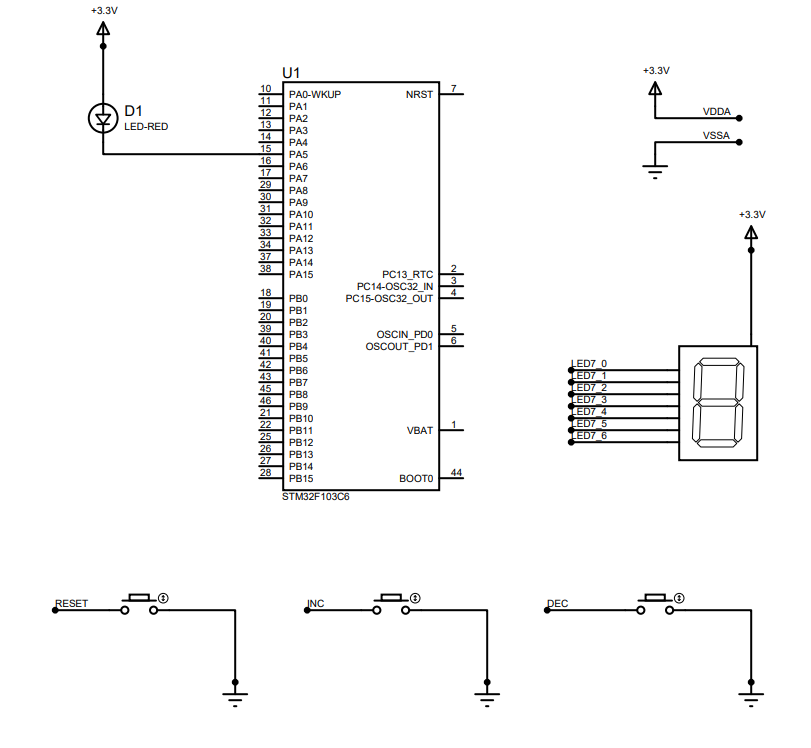
\includegraphics[width=5in]{source/picture/midterm/midtermschematic.PNG}
    \caption{\textit{Proteus schematic for count-down system}}
    \label{project_intro1}
\end{figure}

Một số tính năng chính của hệ thống được trình bày như sau:
\begin{itemize}
    \item LED 7 đoạn dùng để hiển thị giá trị của counter, có giá trị từ 0 đến 9.
    \item Nút \textbf{RESET} được dùng để reset giá trị của counter về 0. Trong khi đó, nút nhấn \textbf{INC} và \textbf{DEC} được dùng để tăng hoặc giảm giá trị của counter. Có 2 sự kiện cần phải xử lý cho các nút nhấn, là nhấn thường và nhấn giữa. Trong dự án này, một nút nhấn được coi là nhấn giữ, nếu nó giữ nguyên trạng thái đó trong 3 giây liên tiếp.
    \item Đèn LED D1 được dùng để theo dõi hoạt động của hệ thống, nó sẽ luân phiên chớp tắt mỗi giây.
\end{itemize}

Sinh viên sẽ hiện thực dự án của mình theo từng bước yêu cầu ở phần bên dưới. Trong mỗi phần, sinh viên cần trình bày các yêu cầu về report. Một số lưu ý quan trọng cho phần hiện thực như sau:

\begin{itemize}
    \item Chu kì của ngắt timer là 10ms. Giá trị của counter khi cài đặt timer có thể là 9 hoặc 10 đều được chấp nhận (trong trường hợp này, prescaller là 7999).
    \item Tất cả các nút nhấn đều được xử lý chống rung bằng ngắt timer 10ms. Một nút nhấn sẽ được xem là nhấn đè nếu nó được giữ liên tục trong 3 giây.
    \item Không sử dụng HAL\_Delay() trong việc hiện thực. Tất cả các hiệu ứng thời gian đều phải được hiện thực dựa trên software timer.
    \item Report này cần được nộp lại kèm theo các câu trả lời của sinh viên.
    \item Link github và video demo trong report này được chỉnh quyền truy cập public.
\end{itemize}

\section{Hiện thực và Report}

\subsection{Sơ đồ nguyên lý trên Proteus - 1 điểm}
Trong phần này, sinh viên đề xuất các kết nối của LED 7 đoạn và 3 nút nhấn với STM32F103C6.\\

\textbf{Report: } Trình bày sơ đồ nguyên lý tại đây. Sinh viên có thể chụp màn hình Proteus cho phần sơ đồ nguyên lý.\\


\subsection{State machine Step 1 - 2 điểm}
Một máy trạng thái sẽ được thiết kế để thực hiện các chức năng với trạng thái nhấn bình thường (normal-press) cho 3 nút nhấn, như sau:
\begin{itemize}
    \item Khi nút RESET is được nhấn, giá trị counter sẽ là 0.
    \item Khi INC được nhấn, giá trị của counter tăng 1 đơn vị. Khi nó đến 9, giá trị tiếp theo là 0.
    \item Khi DC được nhấn, giá trị của counter giảm 1 đơn vị. Khi giá trị của nó là 0, giá trị tiếp theo là 9.
\end{itemize}

Giá trị của biến counter được hiển thị lên LED 7 đoạn.\\

\textbf{Report: } Trình bày máy trạng thái của hệ thống.\\

\textbf{Your report: } Trình bày hiện thực của hàm dùng để hiển thực máy trạng thái ở trên. Thông thường, hàm này sẽ được gọi trong main().

\begin{lstlisting}[caption=Hiện thực máy trạng thái]
void fsm_simple_buttons_run(){
    //TODO
}
\end{lstlisting}

\subsection{State machine Step 2 - 2 điểm}
Trong phần này, việc nhấn giữ (long-press) cho nút INC và DEC được thêm vào trong dự án. Đối với  nút nhấn, sự kiện long-press xảy ra khi nó được nhấn giữ liên tục sau 3 giây.\\

Khi một sự kiện nhấn giữ được phát hiện, giá trị của counter liên tục thay đổi mỗi 1 giây. Ví dụ, giá trị hiện tại của counter là 2. Khi nút INC được nhấn, ngay lập tức giá trị của nó sẽ tăng lên 3. Tuy nhiên, khi INC tiếp tục được giữ, 3 giây sau, sự kiện long-press xảy ra, giá trị của counter tăng lên 4. Từ lúc này, giá trị của counter sẽ tăng lên 1 mỗi giây, cho đến khi nút INC được thả ra. Giá trị của biến counter này được minh họa như hình bên dưới.


\begin{figure}[!htp]
    \centering
    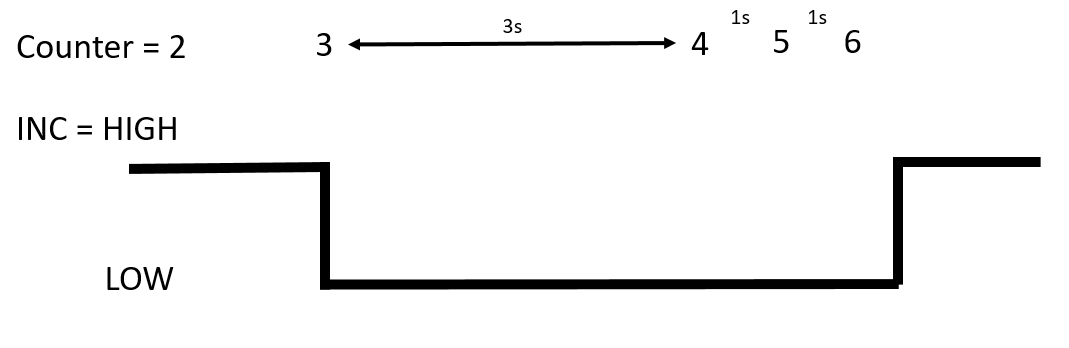
\includegraphics[width=5in]{source/picture/midterm/inclongpress.PNG}
    \caption{\textit{Long press behavior for INC button}}
    \label{longpress}
\end{figure}

Hành vi của nút DEC sẽ ngược lại với nút INC. Giá trị của biến counter sẽ xoay vòng khi nó đến 0 hoặc 9.\\

\textbf{Report: } Trình bày toàn bộ máy trạng thái cho đến bước này.\\

\textbf{Report: } Sinh viên trình bày một hàm chính dùng để hiện thực các trạng thái mới. Các thay đổi trên máy trạng thái cũ không cần phải trình bày ở đây.\\


\subsection{State machine Step 3 - 2 points}
Cuối cùng, khi không có nút nào được nhấn, hệ thống tự động đếm lùi biến counter và dừng lại khi nó bằng 0. Sau đó, nếu nút INC  hoặc DEC được nhấn, trạng thái của hệ thống lại quay về một trong các trạng thái đã thiết kế trước đó.

\textbf{Your report: } Trình bày toàn bộ máy trạng thái, khi sự kiện time-out 10s được thêm vào.\\

\textbf{Report: } Sinh viên trình bày một hàm chính dùng để hiện thực các trạng thái mới. Các thay đổi trên máy trạng thái cũ không cần phải trình bày ở đây.\\\

\subsection{Led Blinky for Debugging - 1 điểm}


Cuối cùng, trong nhiều dự án dựa trên vi điều khiển, có 1 LED luôn luôn chớp tắt mỗi giây, để giám sát hoạt động của hệ thống. Trong project này, LED nối với chân PA5 sẽ được dùng để hiện thực tính năng này.\\

\textbf{Report: } Sinh viên trình bày giải pháp của mình cho tính năng này. Giải pháp có thể rất đơn giản với vài dòng code hoặc thiết kế máy trạng thái và lập trình cho nó. Trong trường hợp thứ 2, sinh viên trình bày máy trạng thái trước khi trình bày phần hiện thực mã nguồn.

\subsection{Github và Demo}

Link github cho dự án của sinh viên được trình bày ở đây, bao gồm tất cả các files trong dự án (configurations, header and source files). Link này là lần commit sau cùng trong project giữa kì của sinh viên.\\



\begin{center}
    \link{Your github link}
\end{center}


Link cho 1 video demo cũng sẽ được trình bày ở phần này.


\begin{center}
    \link{Your video link}
\end{center}



\section{Bài tập thêm - Engineer mindset - 1 điểm}
In this course, we encourage you to obtain an innovative mindset to solve daily problem. In this question, we would expect you to write a C program to solve the following problem. \\

Suffix with Unit\\

EXample:\\

1 suffixWithUnit(123) => 123\\

2 suffixWithUnit(1234) => 1.234 Kilo\\

3 suffixWithUnit(12345) => 12.345 Kilo\\

4 suffixWithUnit(1234567) => 1.234567 Mega\\

5 suffixWithUnit(12345678) => 12.345678 Mega\\


Prototype
\begin{lstlisting}
string suffixWithUnit(double number) {
}
\end{lstlisting}

How would you solve them? Please share your thinking to solve this problem and provide your answer.  


